\documentclass[12pt]{article}
\usepackage{fullpage,enumitem,amsmath,amssymb,graphicx,listings,color,pdfpages,natbib}
\definecolor{mygreen}{RGB}{28,172,0}  % color values Red, Green, Blue
\definecolor{mylilas}{RGB}{170,55,241}

\begin{document}

\begin{center}
{\Large CS221 Fall 2018 Project} \\
{\Large An AI agent for Lunar Lander}

\begin{tabular}{rl}
Collaborators: & Amey Naik, Prabhjot Singh Rai, Abhishek Bharani \\
SU Net IDs: & ameynaik, prabhjot, abharani
\end{tabular}
\end{center}


\section{Introduction}

\noindent\begin{minipage}{0.6\textwidth}
The purpose of this project is to build an AI agent to play Lunar Lander game to safely land on a landing pad. We are making use of Box2D Lunar Lander available on OpenAI gym\citep{openai}. Landing pad is always at coordinates (0,0). Reward for reaching the landing pad is about 100 to 140 points, depending on the speed. If lander moves away from landing pad it loses reward back. Episode finishes if the lander crashes or comes to rest, receiving additional -100 or +100 points. Each leg ground contact is +10. Firing main engine is -0.3 points each frame. Solved is 200 points.
\end{minipage}
\begin{minipage}{0.3\textwidth}\raggedleft
\text{    Figure 1: Game Environment}
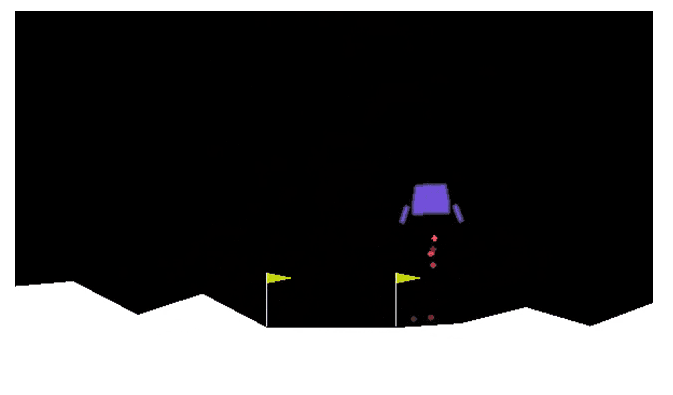
\includegraphics[scale=0.3]{LunarLanderDemoImage.png}
\end{minipage}
\\ \\
Landing outside landing pad is possible. Fuel is infinite. Four discrete actions available: do nothing, fire left orientation engine, fire main engine, fire right orientation engine. Our state at any given frame is defined by 8 parameters: horizontal position (x-axis), vertical position (y-axis), orientation (theta), linear velocity (v), angular velocity (w), state of each landing leg (left and right). Moreover, our environment, which is the surface of the moon, keeps changing with each episode.

\section{Baseline}
We define multiple baselines:
\begin{enumerate}[label=(\alph*)]
\item 
\noindent\begin{minipage}{0.6\textwidth}
Random Action Baseline: Taking random action at any given state out of the available actions. We see that in almost all the cases, we get negative rewards. We also checked if taking a single action leads to the optimum. However this performed worse than taking random actions.
\end{minipage}
\begin{minipage}{0.3\textwidth}\raggedleft
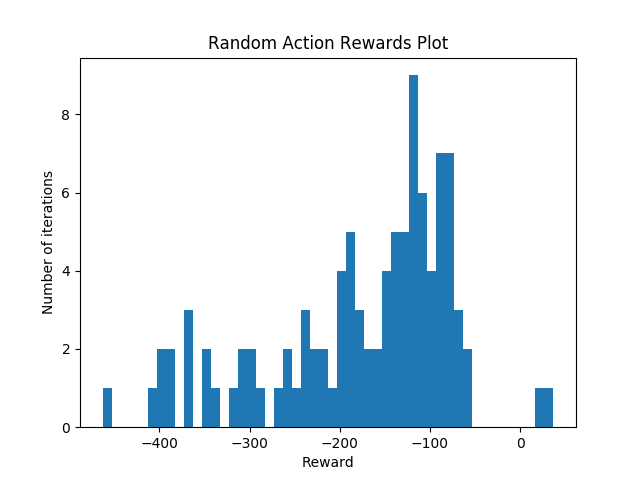
\includegraphics[scale=0.3]{images/random-action-reward-plot.png}
\end{minipage}
\item Start with randomly picking an action for a new state that is explored, if the state gets explored in the episode ‘e1’, then in the next episode ‘e2’ if you encounter that state, pick the previously stored action for that state. Our baseline will be a greedy algorithm which will act to  fetch maximum rewards but does not account for future states and early convergence.
\end{enumerate}


\section{Oracle}
We define multiple oracles for this problem in the increasing order of their performance and complexity:
\begin{enumerate}[label=(\alph*)]
\item Human playing score.
\item Maximum score that one can achieve which is 140 [reach landing pad]  + 100 [stopping without crashing] + 10*2 [each leg ground contact] + 200 [solving the episode]
\end{enumerate}

\section{Metrics}
We can evaluate the performance of agent by comparing the score with the scores from the oracle and in least number of episodes. There is leader-board to compare how fast the learning is of our model against others.\citep{leaderboard}

\section{Challenges And Approach}

Firstly, this problem has a very large state space, we can not expect a simple epsilon-greedy algorithm to explore everything in a reasonable amount of time. The next logical step is to apply Q-learning. This may help us take the best direction but may not provide a detailed planning. In general, it may not understand the game dynamics from a general point of view. By using function approximation, we can generalize well to unseen states. We are planning to explore variants of DQN, particularly DQN with prioritize replay\citep{PrioritizedReplay}, Double DQN\citep{DoubleQ-learning}, and Dueling network architecture\citep{Dueling} to solve this problem.

\bibliography{biblio}
\bibliographystyle{abbrv}

\end{document}